%Input preamble
\documentclass[11pt]{article}

% colors
\usepackage[table]{xcolor}
\definecolor{maroon}{RGB}{153,0,18}
\definecolor{lime}{RGB}{190,213,88}
\definecolor{sand}{RGB}{217,202,179}
\definecolor{fire}{RGB}{144,50,61}
\definecolor{brick}{RGB}{94,11,21}
\definecolor{olive}{RGB}{117,109,84}
\definecolor{lavpink}{RGB}{172,123,132}
\definecolor{darkpurp}{RGB}{49,10,49}
\definecolor{salmon}{RGB}{204,90,113}
\definecolor{mauve}{RGB}{94,73,85}
\definecolor{greyblue}{RGB}{125,132,145}
\definecolor{greypurp}{RGB}{68,56,80}
\definecolor{brightpurp}{RGB}{96,20,255}

% packages (please add in alphabetical order)
\usepackage{adjustbox}
\usepackage{amsfonts}
\usepackage{amsmath}
\usepackage{amssymb}
\usepackage{array}
\usepackage{bm}
\usepackage{booktabs}
\usepackage{caption}
\usepackage{epstopdf}
\usepackage{float}
\usepackage[margin=1in]{geometry}
\usepackage{graphicx}
\usepackage[colorlinks=true, linkcolor=brightpurp, citecolor=brightpurp, urlcolor=salmon]{hyperref}
\usepackage{lipsum}
\usepackage{longtable}
\usepackage{mathtools}
\usepackage{multirow}
\usepackage{natbib}
\usepackage{rotating}
\usepackage{setspace}
\usepackage{subcaption}
%\usepackage{threeparttable}
\usepackage{threeparttablex}
\usepackage{xr}
\usepackage[printwatermark]{xwatermark}


\newcolumntype{L}[1]{>{\raggedright\let\newline\\\arraybackslash\hspace{0pt}}m{#1}}
\newcolumntype{C}[1]{>{\centering\let\newline\\\arraybackslash\hspace{0pt}}m{#1}}
\newcolumntype{R}[1]{>{\raggedleft\let\newline\\\arraybackslash\hspace{0pt}}m{#1}}

% commands
\newcommand{\mr}{\multirow}
\newcommand{\mc}{\multicolumn}

%Other parameters
\newcommand{\noutcomes}{95}
\newcommand{\treatsubsabc}{$75\%$}
\newcommand{\treatsubscarec}{$74\%$}
\newcommand{\treatsubscaref}{$63\%$}

%Counts
%Males
\newcommand{\positivem}{$79\%$}
\newcommand{\positivesm}{$37\%$}

%Females
\newcommand{\positivef}{$73\%$}
\newcommand{\positivesf}{$35\%$}

%Counts, control substitution
%Males
\newcommand{\positivecsnm}{$58\%$}
\newcommand{\positivescsnm}{$25\%$}

\newcommand{\positivecsam}{$74\%$}
\newcommand{\positivescsam}{$38\%$}

%Females
%% no alternative
\newcommand{\positivecsnf}{$83\%$}
\newcommand{\positivescsnf}{$46\%$}

%% alternative
\newcommand{\positivecsaf}{$73\%$}
\newcommand{\positivescsaf}{$23\%$}

%Pooled

%Effects
%Males

%Females
\newcommand{\hsgradf}{$7$}
\newcommand{\yearsedf}{$1.2$}



%Pooled

%CBA
%IRR
%Males
\newcommand{\irrm}{$15\%$}
\newcommand{\irrsem}{$13\%$}

%Females
\newcommand{\irrf}{$10\%$}
\newcommand{\irrsef}{$12\%$}

%Pooled
\newcommand{\irrp}{$13\%$}
\newcommand{\irrsep}{$11\%$}

%BC
%Males
\newcommand{\bcm}{$7.88$}
\newcommand{\bcsem}{$8.06$}

%Females
\newcommand{\bcf}{$2.30$}
\newcommand{\bcsef}{$1.56$}

%Pooled
\newcommand{\bcp}{$4.35$}
\newcommand{\bcsep}{$2.57$}

%NPV streams
%Pooled
\newcommand{\parincomenpvp}{$\$115,026$}

%\interfootnotelinepenalty=10000

\newcommand*\leftright[2]{%
  \leavevmode
  \rlap{#1}%
  \hspace{0.5\linewidth}%
  #2}

\newcommand{\orth}{\ensuremath{\perp\!\!\!\perp}}%
\newcommand{\indep}{\orth}%
\newcommand{\notorth}{\ensuremath{\perp\!\!\!\!\!\!\diagup\!\!\!\!\!\!\perp}}%
\newcommand{\notindep}{\notorth}

\begin{document}

\begin{center}

\singlespacing
\Large \textbf{Early Childhood Education’s Cost-Effective Potential \\ to Improve Life-cycle Outcomes}\\
\bigskip
{\large Jorge Luis Garc\'{i}a}\\
{\large Grace Guthrie Griffith}\\
{\large John E. Walker Department of Economics}\\
{\large Clemson University}

\end{center}
\thispagestyle{empty}

\doublespacing

\noindent Child poverty is a persistent problem in the United States. Investing in comprehensive early childhood education programs is a potentially powerful and cost-effective way to mitigate the negative consequences of child poverty on child development and life outcomes. Short-term follow-ups to the investments document that high-quality early childhood education boosts the skills of disadvantaged children, but new evidence focuses on the long term impact of these programs. This article summarizes four studies which document the positive impact of these programs on multiple domains of human development including reducing the likelihood that participating children will commit crimes or develop chronic diseases later in their lives. The studies show that the improvement of these outcomes is cost-effective, generating an economic return of 7.3 dollars per dollar invested (accounting for the welfare costs of financing the programs through taxation).\\

\begin{sidewaysfigure}[!htbp]
\caption{Net Present Value of Main Components: Life-cycle Evaluation of ABC and CARE}\label{figure:main}
\centering
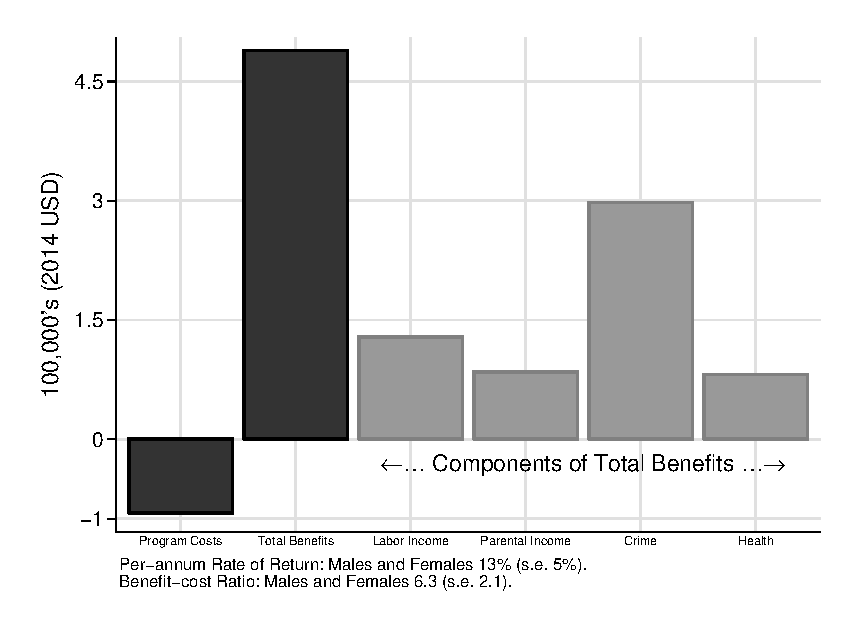
\includegraphics[width=.7\columnwidth]{output/abccare_npvssummredux.eps}
\footnotesize \justify
Source: \citet{Garcia-etal_2018_Quantifying_JPE}.
\end{sidewaysfigure}
	
\noindent \citet{Garcia-etal_2018_Quantifying_JPE} evaluated the \href{https://abc.fpg.unc.edu/abecedarian-project}{Carolina Abecedarian Project (ABC)} and the Carolina Approach to Responsive Education (CARE), two early childhood education programs which supplemented the family by promoting skills such as language and cognitive development. The treatment group was enrolled at 8 weeks of age until age 5 for 50 weeks  per year. The authors monetize the treatment effects of the the measured benefits and costs to participants over their lives. Figure~\ref{figure:main} displays the average life-cycle net present values per program participant of the main components of the benefit/cost analysis of ABC/CARE (program costs, total benefits---labor income, parental labor income, cost of crimes, and quality-adjusted life years) from birth to forecasted death, discounted to birth at a rate of 3\%.\\

\begin{sidewaysfigure}[!htbp]
\centering
\caption{Treatment Effects of ABC and CARE}\label{fig:labor-income-profiles}
\begin{subfigure}[h]{0.5\textwidth}
		\centering
		\caption{Crime} \label{fig:crime}
		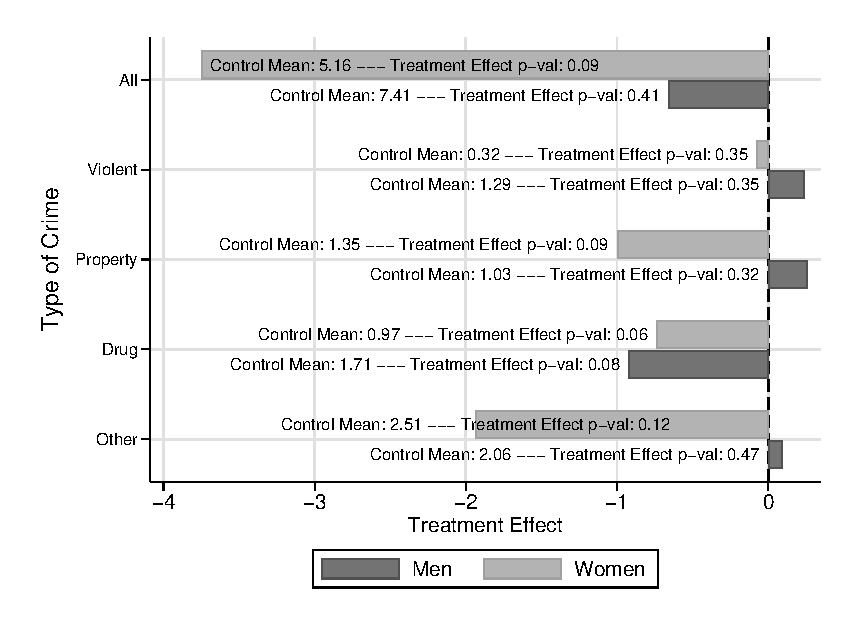
\includegraphics[width=\textwidth]{output/abc-crime-tes-bygender2}
\end{subfigure}%
\begin{subfigure}[h]{0.5\textwidth}
		\centering
		\caption{Health} \label{fig:health}
		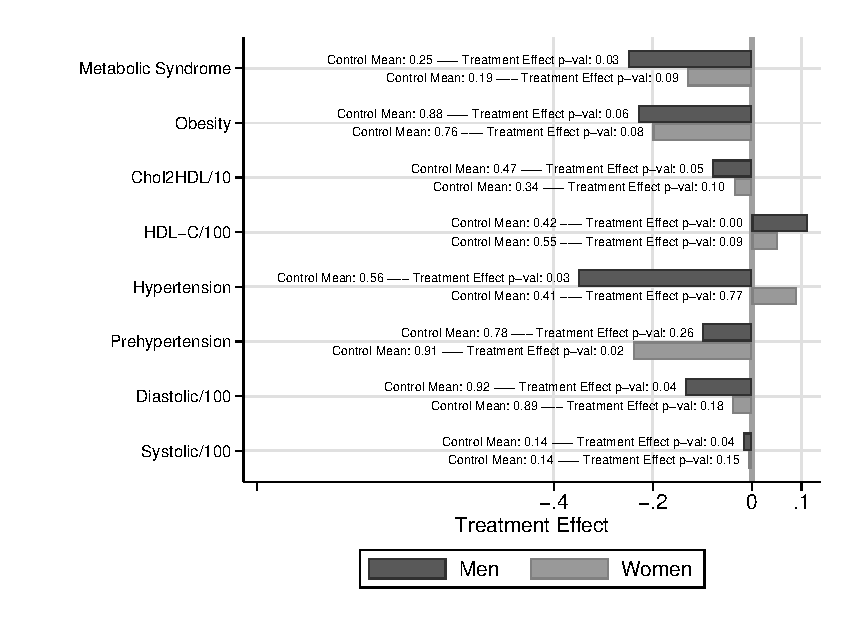
\includegraphics[width=\textwidth]{output/healthtes}
\end{subfigure}
\footnotesize \justify
\item Source: \citet{Garcia_etal_2019_ECE_IMHJ} and \citet{Garcia_Heckman_2019_Early_HE}. 
\end{sidewaysfigure}

\noindent Figure~\ref{figure:main} indicates that crime is a significant part of the benefit of the program, so \citet{Garcia_etal_2019_ECE_IMHJ} further investigated it using criminal administrative records. Figure~\ref{fig:crime} from \citet{Garcia_etal_2019_ECE_IMHJ} displays the treatment effects separately for men and women across crime categories. Across all of the crime outcomes, there is a positive treatment effect for females for all outcomes (property, violent, and drug crimes); for males, there is a positive treatment effect for only drug crimes. Therefore, as noted by \citet{Garcia_Heckman_Ziff_2018_EER}, there is considerable evidence that the effect of early childhood education programs differs according to gender. Weighting the treatment effects on crime by the costs rather than the quantity of the crimes reveals a different pattern. The benefit of the reduction in male crimes (\$466,318 2017 USD) is much larger than the benefit of the reduction in female crimes (\$32,790 2017 USD). As a consequence of the program, men substantially decreased their participation in crimes that are very costly to society. \\ 

\noindent In addition to reducing crime, \citet{Garcia_Heckman_2019_Early_HE} found that early childhood education programs can reduce the likelihood that participants will develop chronic diseases. The treatment effects displayed in Figure~\ref{fig:health} from \citet{Garcia_Heckman_2019_Early_HE} were measured when participants were in their mid-30s. These early-adulthood treatment effects lead to reduced incidence of heart disease, stroke, cancer, and mortality across the life-cycle of participants of both genders. The female treatment group has a slightly lower mortality rate than the control group. Male mortality rates diverge over time between treatment and control, but control males are nearly four times more likely to die than treatment males by age 75. Quality-adjusted life years (QALYs) measure the value of health outcomes, combining the quality and the quantity of life into an index number. For males, the increase in QALYs more than offsets all program costs (including the welfare costs of financing the program through taxation) and the increase in QALYs offsets nearly half of the program’s costs for females.\\

\noindent The series of articles concludes with a cautionary note that we echo here. ABC/CARE was implemented in a relatively disadvantaged and predominately African-American population in a university town in North Carolina. The generalization of its findings to other populations may be unwise. In particular, there is no basis for using the studies to argue for universal application of ABC/CARE across all socio-economic groups despite its cost effectiveness. By studying the features of ABC/CARE, we can begin to determine what cost effective early childhood education programs may benefit disadvantaged populations (who have the largest potential to benefit from these programs).


%References
\singlespace
\bibliographystyle{chicago}
\bibliography{heckman}

\end{document}

